\documentclass{article}%
\usepackage[T1]{fontenc}%
\usepackage[utf8]{inputenc}%
\usepackage{lmodern}%
\usepackage{textcomp}%
\usepackage{lastpage}%
\usepackage[head=40pt,margin=0.5in,bottom=0.6in]{geometry}%
\usepackage{graphicx}%
%
\title{\textbf{Los presos políticos que han muerto en las instalaciones del Sebin}}%
\author{El Nacional Web}%
\date{08/10/2018}%
%
\begin{document}%
\normalsize%
\maketitle%
\textbf{URL: }%
http://www.el{-}nacional.com/noticias/presos{-}politicos/los{-}presos{-}politicos{-}que{-}han{-}muerto{-}las{-}instalaciones{-}del{-}sebin\_254931\newline%
%
\textbf{Periodico: }%
EN, %
ID: %
254931, %
Seccion: %
Presos políticos\newline%
%
\textbf{Palabras Claves: }%
Sucesos, Gobierno\newline%
%
\textbf{Derecho: }%
1.1%
, Otros Derechos: %
1.2%
, Sub Derechos: %
1.1.1.3, 1.2.2%
\newline%
%
\textbf{EP: }%
NO\newline%
\newline%
%
\textbf{\textit{El concejal del municipio Libertador, Fernando Albán, se convierte en la tercera persona que muere en el centro penitenciario}}%
\newline%
\newline%
%
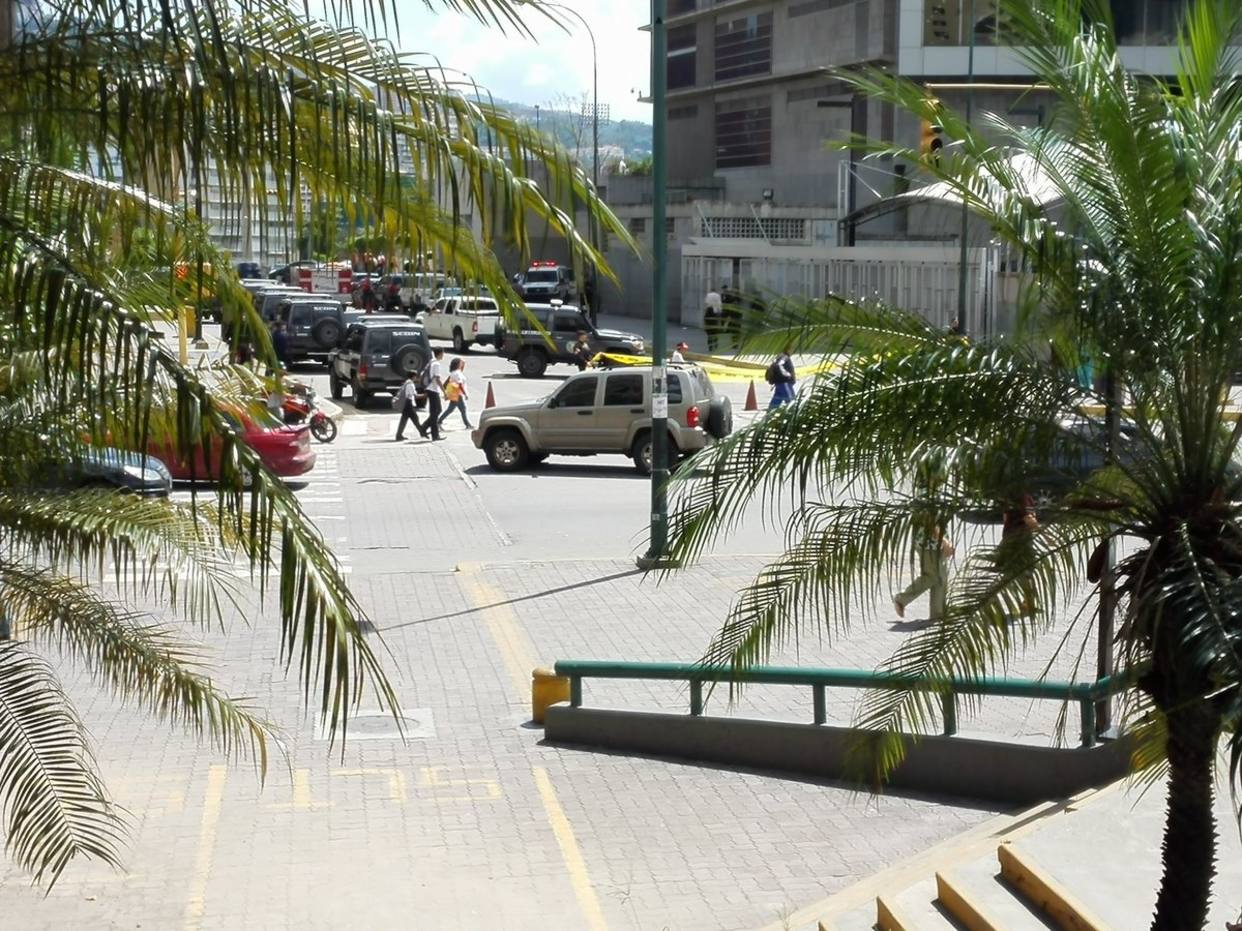
\includegraphics[width=300px]{75.jpg}%
\newline%
%
Tres representantes~opositores han muerto en el Servicio Bolivariano de Inteligencia (Sebin), ubicado en Plaza Venezuela, durante los últimos tres años.~La muerte del concejal del municipio Libertador, Fernando Albán, se convierte en la tercera~que ocurre~en las instalaciones del mencionado organismo. En todos los casos, el sector opositor responsabilizó al gobierno de Nicolás Maduro.%
\newline%
%
13 de marzo de 2015%
\newline%
%
Rodolfo González,~piloto de la aviación civil venezolana,~murió~por presuntamente ahorcarse en la celda en El Helicoide, luego de estar preso~desde el 2014. González, de 63 años de edad,~ fue detenido bajo la acusación de asociación para delinquir bajo la tenencia de explosivos y tráfico de armas de fuego y por su~presunta~vinculación con los hechos violentos que iniciaron en febrero del citado año.%
\newline%
%
José Vicente Haro, abogado~constitucionalista y representante legal del piloto, detalló que una fuente interna del Sebin le informó que~“fue encontrado ahorcado, decidió suicidarse luego de haberse enterado que sería trasladado a una cárcel común”, reseñó~El Tiempo.%
\newline%
%
17~de septiembre de 2017%
\newline%
%
Carlos Andrés García, concejal de Guasdualito, estado Apure,~falleció~luego de sufrir un ACV mientras se encontraba ~detenido en~la sede del Servicio Bolivariano de Inteligencia Nacional (Sebin).%
\newline%
%
El partido político Primero Justicia aseguró que el concejal fue detenido ilegalmente y le fue~negada la~atención médica. La coalición opositora aseguró que~cuando García fue trasladado a un centro médico~~“ya no había posibilidad de hacer nada para mejorar su salud”.%
\newline%
%
A García se le había otorgado la medida cautelar de casa por cárcel dos días antes de su muerte.~Sin embargo, la orden nunca fue ejecutada.%
\newline%
%
8 de octubre de 2018%
\newline%
%
El concejal del municipio Libertador en Caracas,~Fernando Albán,~fue detenido el viernes 5 de octubre en el aeropuerto Internacional Simón Bolívar en Maiquetia, Vargas, cuando regresaba de una visita familiar en Estados Unidos.%
\newline%
%
Tarek William Saab, fiscal general designado por la asamblea nacional constituyente,~informó que había sido detenido por estar presuntamente implicado en el atentado contra el presidente~Nicolás Maduro~del pasado 4 de agosto.%
\newline%
%
En relación con el caso, existen dos versiones oficiales:%
\newline%
%
Saab~indicó~que~Albán~pidió ir al baño y luego se lanzó desde el~piso 10 del establecimiento.%
\newline%
%
Néstor~Reverol,~ministro de Relaciones Interiores, Justicia y Paz, afirmó~que el representante municipal~estaba en la sala de~espera para ser trasladado a los Tribunales cuando se lanzó por una ventana del centro de detención.%
\newline%
%
Desde su aprehensión, los funcionarios del Sebin lo mantuvieron incomunicado~con sus familiares. No explicaron los motivos de~ su detención y tampoco confirmaron dónde se encontraba Albán.%
\newline%
%
Se esperaba que la presentación ante los tribunales de Albán fuese el domingo 7 de octubre. Este acto procesal no se realizó.%
\newline%
%
El presunto cadáver del diputado fue hallado en las adyacencias de la sede del Sebin en Plaza Venezuela.%
\newline%
%
\end{document}